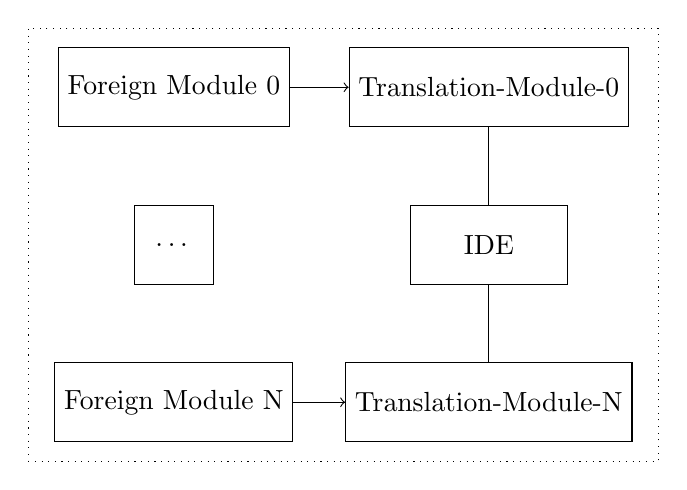
\begin{tikzpicture}
  % Nodes
  \node (b) [rectangle, draw, minimum height=5.5cm, minimum width=8cm, dotted] at (-2.85, 0) {};
  \node (p-0) [rectangle, draw, minimum height=1cm, minimum width=2cm] at (-5, 2) {Foreign Module 0};
  \node (dots) [rectangle, draw, minimum height=1cm, minimum width=1cm] at (-5, 0) {\dots};
  \node (p-n) [rectangle, draw, minimum height=1cm, minimum width=2cm] at (-5, -2) {Foreign Module N};
  \node (m-1) [rectangle, draw, minimum height=1cm, minimum width=2cm] at (-1, 2) {Translation-Module-0};
  \node (m-n) [rectangle, draw, minimum height=1cm, minimum width=2cm] at (-1, -2) {Translation-Module-N};
  \node (i) [rectangle, draw, minimum height=1cm, minimum width=2cm] at (-1, 0) {IDE};
  % Arrow
  \draw (m-1.south) -- (i);

  \draw (m-n.north) -- (i);

  \draw[->] (p-0) -- (m-1);
  \draw[->] (p-n) -- (m-n);
\end{tikzpicture}
